
\newpage
\section{Agent-Based Foraging Model}

\subsection{Methods}

\subsubsection*{Main Features} %Assumptions
The model was developed based on empirical findings for foraging rules and pollinator behavior.  It is a simple spatial model of two co-flowering plant species competing over pollination service. 

In the model, all pollinators (from now on called "bee-agents") are identical and the two flower types only differ in their species identity. Reward replenishment, handling times to extract the reward and its attractiveness towards the bee-agents is identical for both species. Corolla color is only assigned for better visualization and is not important for the model or the bee-agents, respectively. All bee-agents behave under the hypothesis of flower constancy which is empirically tested for various pollinators (e.g. \citet{hill1997spontaneous} for honey bees, \citet{chittka1997foraging} for bumble bees, \citet{goulson1998flower} for hoverflies and \citet{goulson1997foraging} for the butterfly \textit{Thymelicus flavus}). Flower constancy is the tendency of an individual pollinator to keep visiting the same flower species instead of switching to more rewarding or closer species \citep{chittka1999flower,waser1986flower}. Because we are interested in the visitation rate of flowers in different frequencies, the energetic costs and the limit of gained rewards of the bee-agents are ignored. Furthermore, they do not communicate and always empty a flower completely. 
%Solitär, unlimited nectar

\subsubsection*{Model Environment}
I used NetLogo \citep{wilensky1999netlogo} as programming environment. It is a simple but powerful tool for making ABMs and connectible with R through the R-package "RNetLogo" \citep{thiele2014r}. In NetLogo, the "world" is a spatial grid with a set number of cells called patches. Agents can move freely over the patches according to their given behavior rules. Patches and agents both have own properties and can interact with each other. 
In my model, the "meadow" has 100x100 grid cells with horizontally and vertically wrapping to avoid edge effects. Every grid cell can either contain a single flower of one of the two species or grass. 

Figure~\ref{fig:cluster} shows a set of exemplary model environments. Floral cover is defined as the percentage of the patches containing flowers and the cluster number equals the average number of flowers within a cluster. The number of clusters per species can be calculated by dividing the number of flowers per species on the meadow through the cluster number. If the cluster number is one, all flowers are randomly distributed over the meadow. With increasing cluster size, one flower per cluster is assigned on the meadow ("cluster-seeds") and all remaining flowers of that species are randomly allocated to them in a second step.

Every flower contains 1 Joule of reward in the beginning of each simulation run. The bee-agents are randomly distributed over the modeling environment and start without a fixed preference for a flower type but just pick the closest one when the simulation starts. Every time step in NetLogo equals one second. 


\begin{figure} [!ht] % screenshots
	\centering
	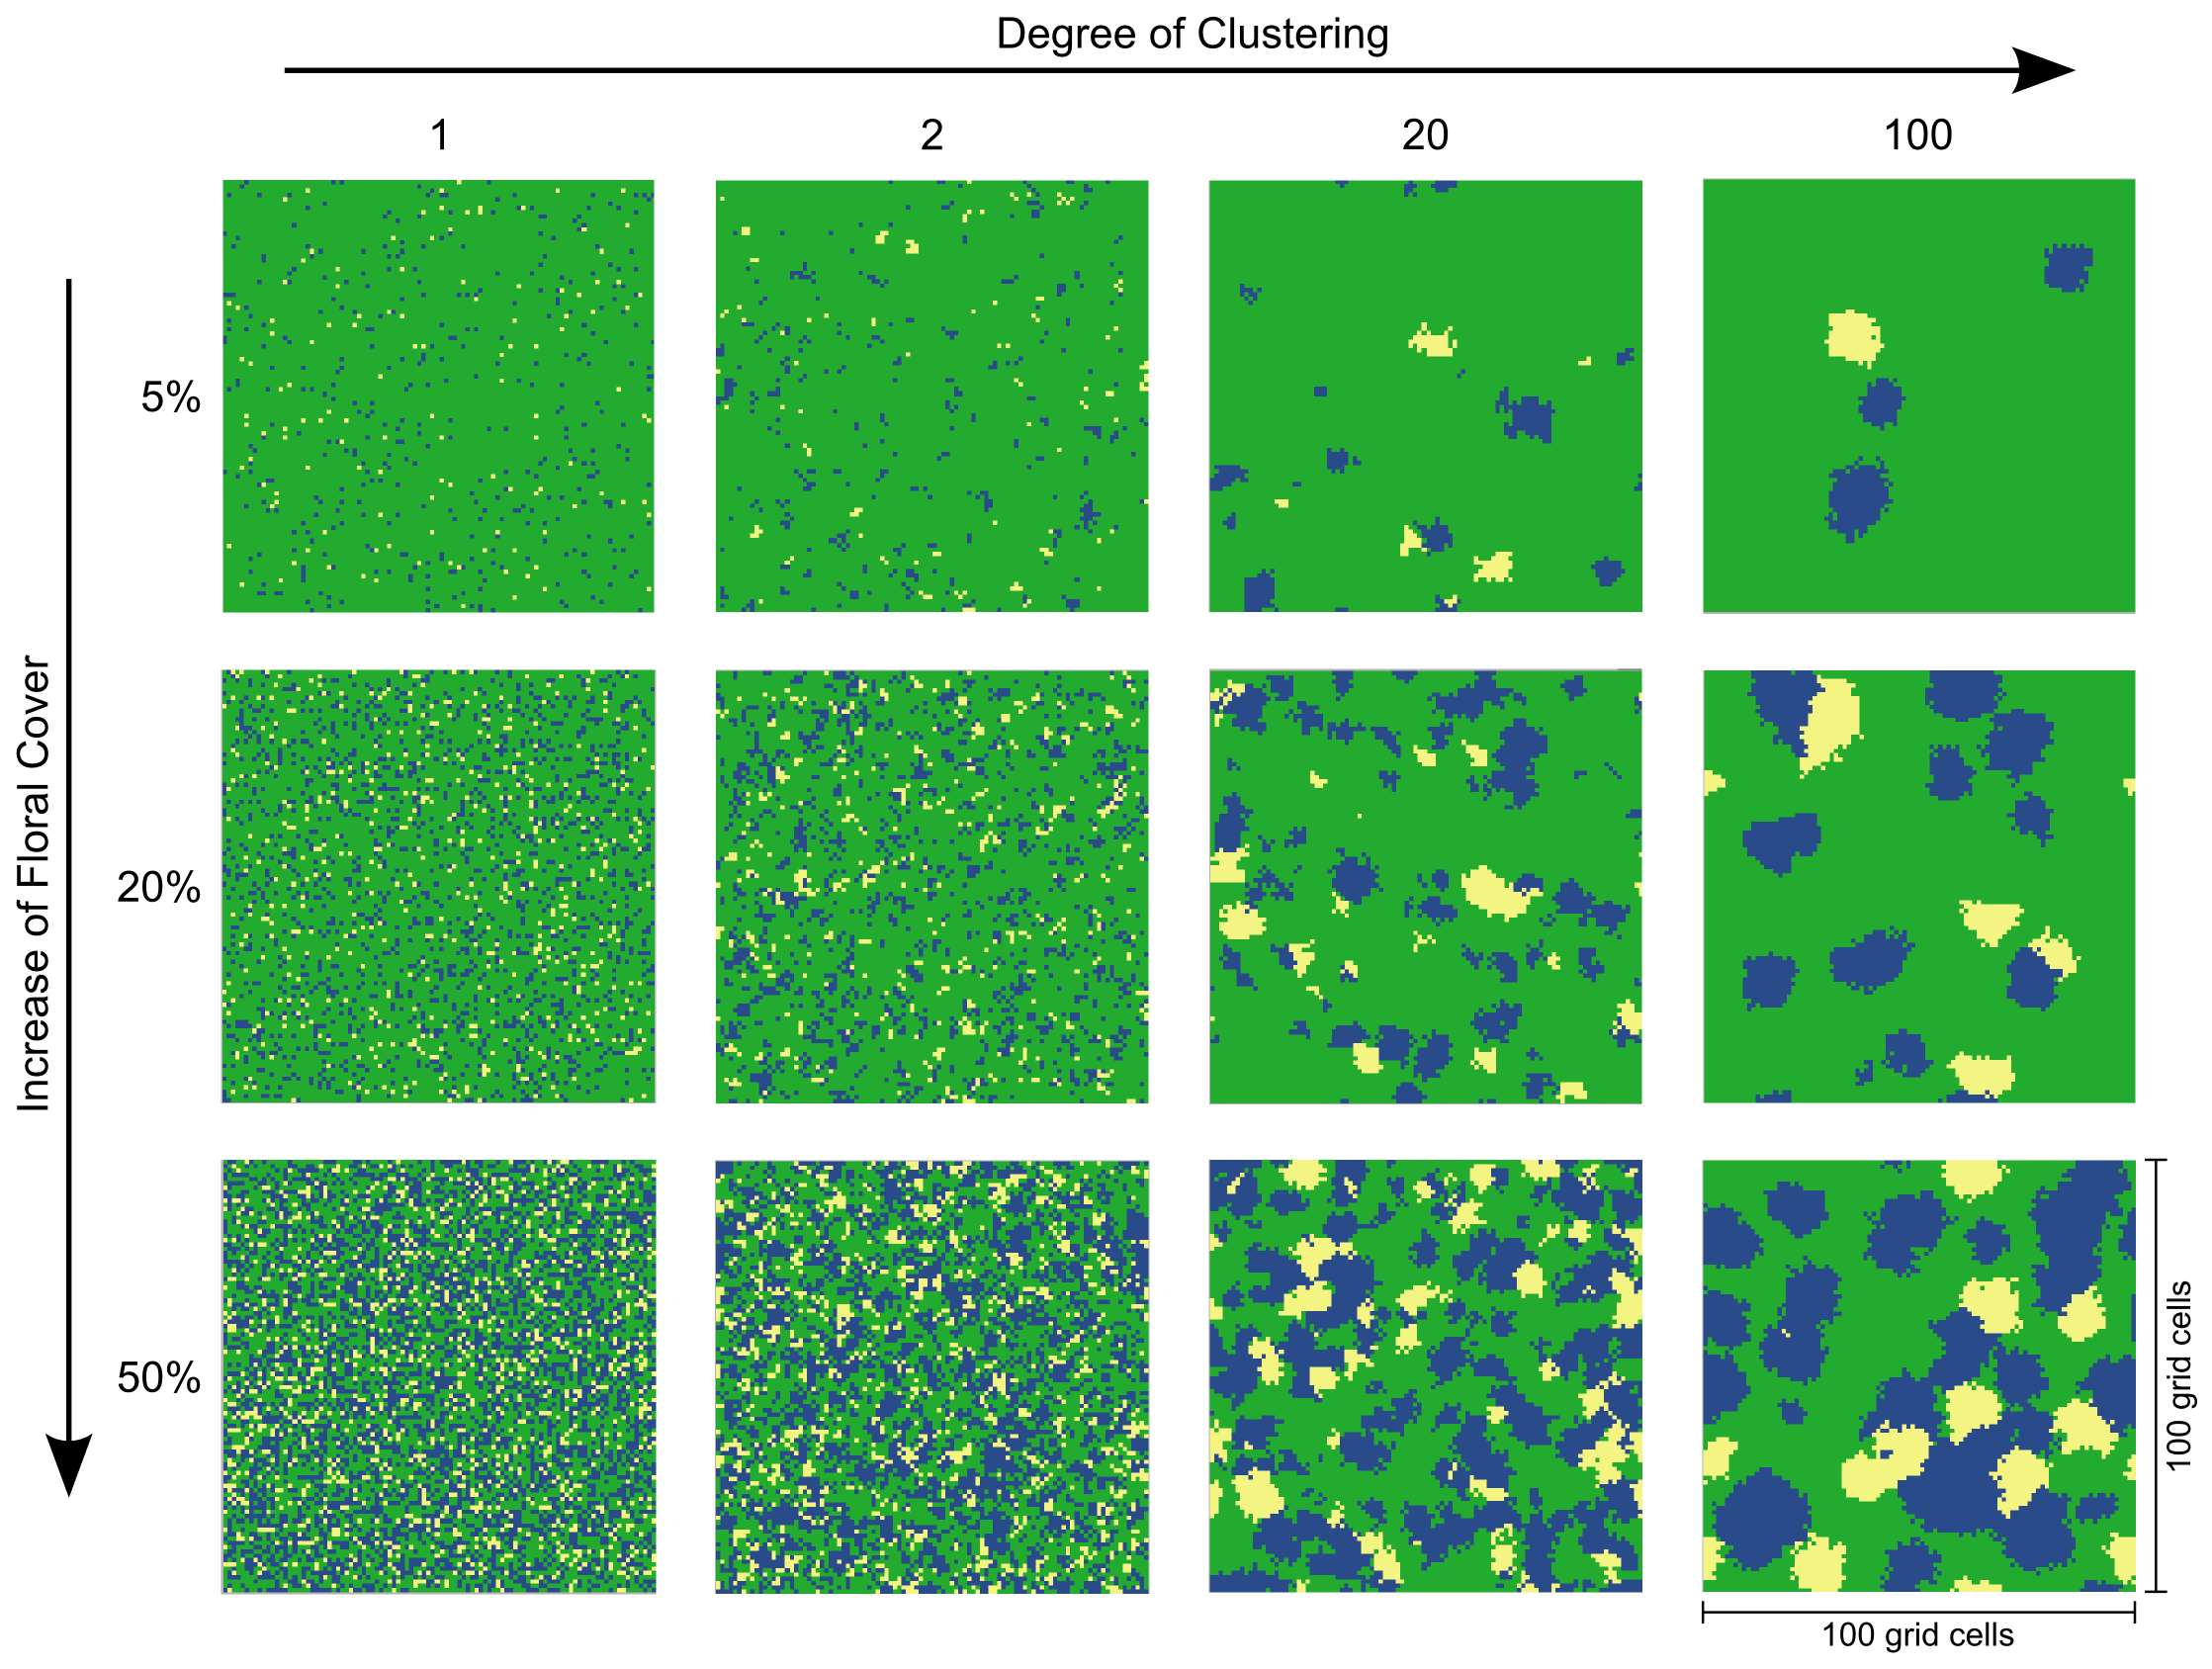
\includegraphics[width=14cm]{Images/cluster}
	\caption{ Exemplary model environment setups with increasing floral cover and cluster size. The cover expresses the percentage of patches containing a flower ($\Sigma_{patches}$ = 10 000). The cluster number equals the average amount of flowers per cluster. Flowers are randomly assigned to the clusters in the model setup. }
	\label{fig:cluster}
\end{figure}


\subsection*{Behavior Rules}

All bee-agents act independently from each other according to the behavior rules shown in Figure~\ref{fig:flowchart} (Overview of all parameters used for the model with its default settings in the supplementary material in tab.~\ref{tab:parametervalues}).  

As mentioned in the assumptions, the behavior of the bee-agents is strongly influences by flower constancy ( e.g. \citealp{bobisud1975pollinator, chittka1997foraging, thomson1981field, chittka1999flower,  goulson1994model,  goulson1999foraging}). Bee-agents always prefer of one of the two flowering species and forage exclusively on this species. The preference can change due to lack of searching success or a series of low rewards of the preferred flower \citep{chittka1997foraging,kunin1993sex,greggers1993memory}. At any given time, a bee-agent can be in one of two states: search for a flower or visit one. 


\begin{figure} [!ht] %flowchart
	\centering
	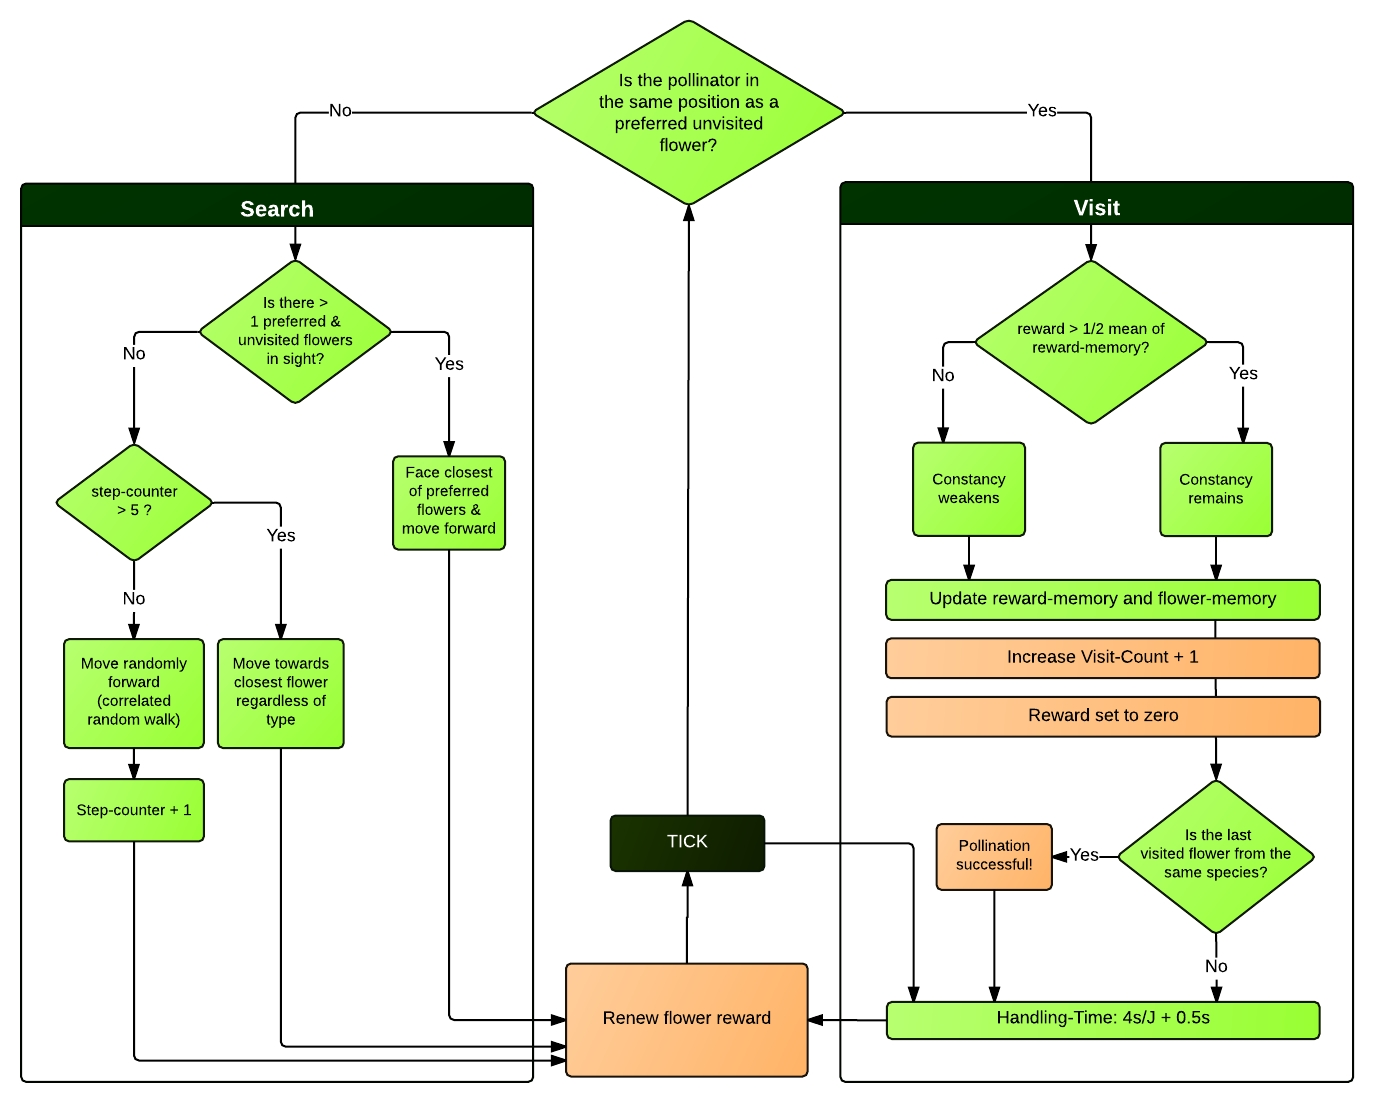
\includegraphics[width=14cm]{Images/flowchart-model}
	\caption{Flowchart describing the behavior rules for the bee-agents within the agent-based model. At any time given, a bee-agent can either search for a preferred flower or visit one. While searching, a bee-agent can remember the location of the last four visited flowers to avoid double-encountering. If there is no flower in sight after 5 seconds of correlated random walk (CRW), the probability that it will encounter the next available flower despite its type increases by 10\% per additional time step. When a bee-agent visits a flower it takes all reward within a reward-dependent handling time and compares the amount with its memory. If the reward is low, the agent is more likely to visit the other flower type next time. The maximum of visits within a successful pollination is possible (x) is determined by the pollen carryover parameter.}
	\label{fig:flowchart}
\end{figure}


\subsubsection*{Search}

Pollinators avoid recently visited flowers \citep{goulson1999foraging}. Every bee-agent possesses with a memory to remember the location of the last four already visited flowers \citep{goulson2000pollinators}. 
 If there is any not recently visited and preferred flower in sight, the searching bee-agent moves directly towards the flower, otherwise it continues searching. 

Previous research on the speed of foraging pollinators by \cite{essenberg2012explaining} and \cite{kunin1991few} (in  \citealt{kunin1996pollinator}) gives 0.1m/sec as benchmark. Consequently, bee-agents can move 1 grid cell per time step in this model. The vision of pollinators was studied in various experiments using a Y-maze apparatus \citep{dyer2008comparative, wertlen2008detection, ne2001effect}. Every bee-agent can detect flowers from a distance of 0.7m with an equivalent of 6 grid cells. The vision is reduced to a 180$^{\circ}$ cone-shaped field to the front of the agent. Pollinators tend to keep their direction while foraging \citep{waddington1980flight}. In the model, I used a correlated random walk (CRW) to achieve a relatively natural movement \citep{bartumeus2005animal, codling2008random,  pyke1992flight, viswanathan2008levy}. Empirical studies have shown an increasing probability to abandon the original flower preference the longer the search remains unsuccessful \citep{chittka1997foraging,kunin1993sex}. If the bee-agent searches for 5 seconds (= 5 time steps) without finding any preferred and unvisited flower, the likelihood of changing its preference increases by 10\% with every additional time step. \\

\subsubsection*{Visit and Reward Intake}

When a bee-agent encounters a preferred and unvisited flower it takes up all its reward. As long as the reward content of a flower lower than the maximum it is refilled by 0.00004 Joule in each time step until the maximum of 1 Joule is reached (see "reward-function" in tab.~\ref{tab:parametervalues}). The handling time of a bee-agent visiting a flower involves three components: a time proportional to the amount of reward taken, a reward-independent constant and a skill factor \citep{kunin1996pollinator}. In my model, a bee-agent requires 4 seconds to extract one Joule of reward plus a reward-independent handling time of 0.5 seconds. When the bee-agent just changed its flower preference it gets a 3 second penalty for inexperience (\citealt{roubik1992ecology}, \citealt{kunin1996pollinator}).

The reward taken is stored in each individual's reward-memory. Every agent can remember the last four rewards received. When visiting a flower, the bee-agent compares this memory with the current reward quantity. If the reward is less than half the average in the memory, the likelihood to abandon flower constancy and visit the other species next increases by 10\%. If the reward is exceptionally good (at least twice the remembered average), the change probability is set to zero  \citep{chittka1997foraging, keasar1996innate}. 

Additional to the quantity of visits we're also interested in their quality. A flower can only be successfully pollinated if the bee-agent visited the same species before. The maximal number of heterospecific flower visits which still allows successful pollination is determined by the degree of pollen carryover. The parameter applies to all bee-agents and can have a value between 1 and 16. For the value of one, the very last visit has to be from the same species (strong heterospecific pollen interference, see \citealt{campbell1986predicting,benadi2012population,montgomery2009pollen}).

After reward-collection is completed, the bee-agent updates its flower-memory and its reward-memory and continues foraging. Each visit and successful pollination is recorded for later analysis. 


\subsection*{Simulation experiments}

Parameters altered in the main analysis are frequency, floral cover, degree of clustering and pollen-carryover. Each parameter-combination was run 20 times with a length of 1000 ticks each (110,400 runs in total). Additionally, I performed a sensitivity analysis with additional parameters which affect the behavior of the bee-agents to understand how the values of these parameters influence the frequency dependence of per-flower visitation rate. Table~\ref{tab:simulation_run} presents the definition and value range of the parameters.
 
\begin{table} [!htbp] %parameter values
	\centering
	\caption{Parameter values used for the main and sensitivity analysis. Only general parameters were changed in the main analysis, whereas the sensitivity analysis also directly influences the behavior of the bee-agents. Each combination was repeated 20 times for 1000 time steps, that makes a total of 110,400 runs in the main analysis and 16,560 runs for each parameter of the sensitivity analysis. }
	\begin{tabular} {l l l}
		\toprule
		\textbf{Parameter} & \textbf{Description}  & \textbf{Values}\\
		\midrule
		\addlinespace[0.2cm]
		\multicolumn{ 3} {l} {\textsc{Main analysis}} \\ 
		\addlinespace[0.2cm]
		Frequency & Proportion of species A on all flowers  & 0-100\% (5\%-steps)\\
		Flower cover & Proportion of patches containing a flowers  & 5, 10, 20, 50 \%\\
		Degree of clustering & Average number of flowers per cluster   &  1, 2, 5, 10, 20, 50, 75, 100\\
		Pollen carryover & Number of visits within a successful pollination is possible & 1, 2, 4, 6, 8, 16\\
		
		\addlinespace[0.2cm]
		\multicolumn{ 3 } {l} {\textsc{Sensitivity analysis}} \\ 
		\addlinespace[0.2cm]
		Reward function & Increase of reward per flower and second & 0, 0.00004, 0.001, 0.1 J/sec \\
		Vision distance & Range of patches within a bee-agent can detect flowers & 1, 6, 20, 50 patches\\
		Search time & \begin{tabular}{@{}l@{}} Number of seconds a bee-agent searches before\\ the probability of switching flowers increases \end{tabular}   & 1, 5, 20, 50 sec \\
		Pollinator density & Number of bee-agents on the meadow & 5, 10, 20, 50 bees\\
		
		\bottomrule
	\end{tabular}
	\label{tab:simulation_run}
\end{table}

